\documentclass[border=10pt]{standalone}

\usepackage{tikz}
\usepackage{verbatim}
\usetikzlibrary{arrows.meta}
\usetikzlibrary{arrows,shapes,chains}

\tikzstyle{base} = [rectangle, rounded corners, draw=black, minimum width=4cm, minimum height=1cm, text centered, font=\sffamily]
\tikzstyle{activityStarts} = [base, fill=blue!30]
\tikzstyle{startstop} = [base, fill=red!30]
\tikzstyle{activityjudge} = [diamond, rounded corners, draw=black,minimum width=4cm, minimum height=1cm, text centered, font=\sffamily,fill=green!30]
\tikzstyle{process} = [base, minimum width=2.5cm, fill=orange!15, font=\ttfamily]

\begin{document}

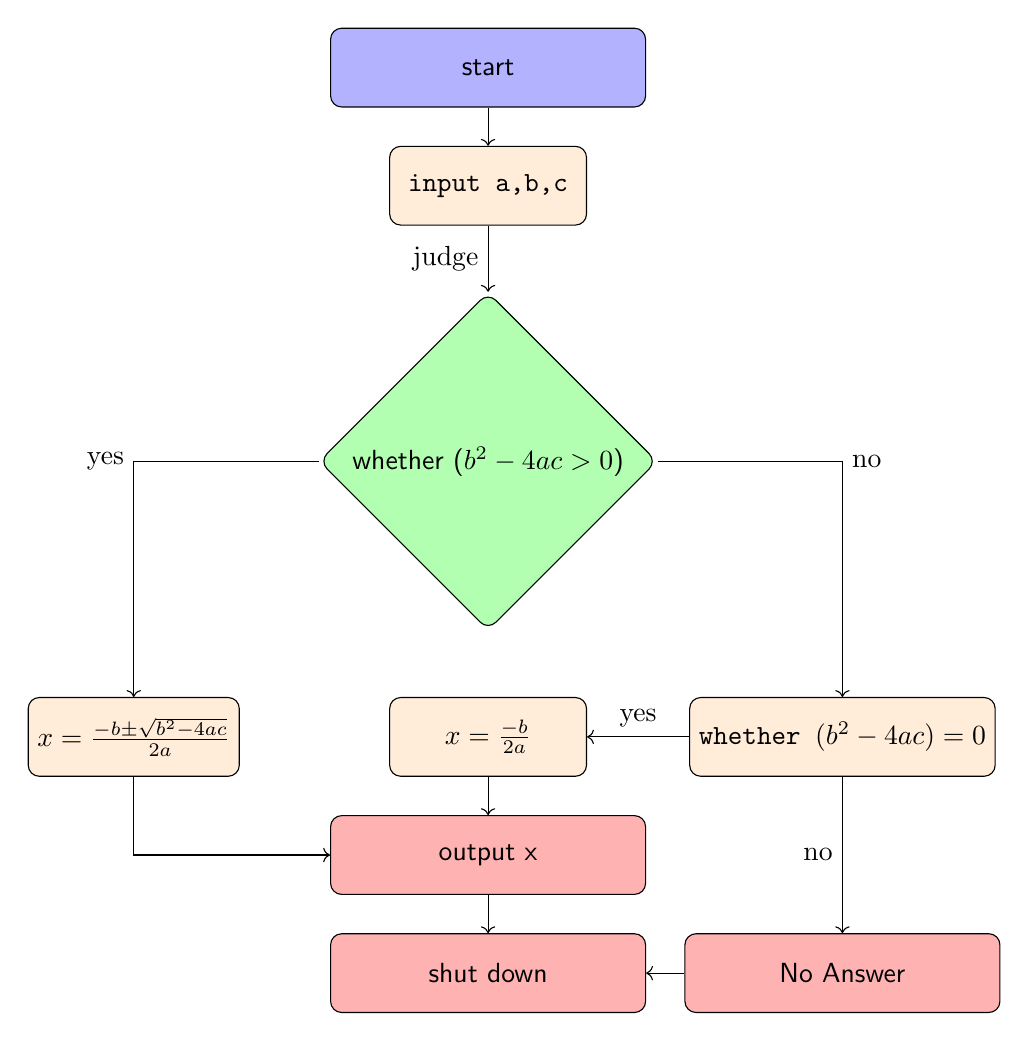
\begin{tikzpicture}[node distance=1.5cm]%, every node/.style={fill=white, font=\sffamily}, align=center]
  \node (start) [activityStarts]  {start};
  \node (input) [process, below of=start] {input a,b,c};
  \node (if1)   [activityjudge, below of=input, yshift=-2cm]   {whether ($b^2-4ac > 0$)};
  \node (X)     [process, below of=if1,yshift=-2cm]   {$x=\frac{-b}{2a}$};
  \node (output)      [startstop, below of=X] {output x};
  \node (if2)      [process, right of=X, xshift=3cm] {whether $(b^2-4ac) = 0$};
  \node (X12) [process, left of=X, xshift=-3cm] {$x = \frac{-b \pm \sqrt{b^2-4ac}}{2a}$};
  \node (stop) [startstop, below of=output] {shut down};
  \node (NO) [startstop, right of=stop, xshift=3cm] {No Answer};
  
  \draw[->] (start) -- (input);
  \draw[->] (input) -- node[anchor=east] {judge} (if1);
  \draw[->] (if1) -| node[anchor=west] {no} (if2);
  \draw[->] (X) -- (output);
  \draw[->] (output) -- (stop);
  \draw[->] (if1) -| node[anchor=east] {yes}(X12);
  \draw[->] (if2) -- node[anchor=south] {yes} (X);
  \draw[->] (if2) -- node[anchor=east] {no} (NO);
  \draw[->] (X12) |- (output);
  \draw[->] (NO) -- (stop);
\end{tikzpicture}

\end{document}
